\chapter{Implementación}

\section{Implementación de la Vista}

\subsection{Herramientas para el desarrollo}

Para la programación del sitio web se ha hecho uso de los lenguajes de programación HTML, CSS, y Javascript. En concreto, se ha utilizado HTML5 y CSS3.

Adicionalmente, se han empleado recursos varios, como pueden ser imágenes extraídas de Internet y un \gls{plugin} para la creación de ventanas emergentes, SweetAlert2 \footnote{\url{https://sweetalert2.github.io}}. En concreto, este \gls{plugin} lo forman dos archivos extraídos del repositorio de la aplicación en JSDelivr \footnote{\url{https://www.jsdelivr.com/package/npm/sweetalert2}}. Como se puede ver en esta página, la versión empleada de SweetAlert2 es 11.4.17. Los dos archivos se guardan una carpeta concreta llamada plugin que se encuentra junto a la carpeta de imágenes y la carpeta de scripts de Javascript.

\subsection{Interfaz responsive}

Una interfaz responsive es un tipo de interfaz que se adapta al dispositivo donde se esté visualizando el sitio web. Para crear estas interfaces responsive se crean distintos estilos CSS dependiendo del dispositivo, en concreto dependiendo del tamaño de su pantalla. Esta filosofía de creación de sitios web permite generar varios sitios web, definiendo una única vez los elementos que forman el sitio web y definiendo varios estilos que modifiquen los atributos de esos elementos, permitiendo el acceso a un mayor volumen de usuarios al no limitar los dispositivos con los que se puede acceder al sistema. Para obtener más detalles sobre las interfaces responsive de nuestro sistema puedes ver el Apartado \ref{sec:def_interfaces_responsive}.

\subsection{Modo oscuro}

Hasta hace pocos años los sitios web únicamente tenían implementados temas claros, es decir, la tonalidad de la página web se torna a colores más claros y el texto a colores más oscuros. Últimamente, se han empezado a usar masivamente los temas oscuros, que son totalmente lo contrario a los temas claros. Definir ambos temas es sencillo, pero hace falta un mecanismo para pasar de un tema a otro de forma intuitiva y sencilla para el usuario.

El mecanismo usado para cambiar de tema es un interruptor. Este interruptor tiene dos estados, uno para cada tema. Visualmente, el estado del interruptor se muestra distinto en modo inactivo (
\includegraphics[width=0.07\textwidth]{imagenes/07_Implementacion/switch_inactive.png}) que en modo activo (
\includegraphics[width=0.07\textwidth]{imagenes/07_Implementacion/switch_active.png}).

Este interruptor se encontrará en la barra de navegación de cada una de las secciones de nuestro sitio web. Para obtener más información sobre el funcionamiento y la implementación del interruptor puedes consultar el Apartado \ref{sec:funcio_interruptor}.

\subsection{Menú lateral}

Esta funcionalidad forma parte de las interfaces responsive, ya que en algunos dispositivos el ancho de la pantalla no es lo suficientemente amplio como para mostrar toda la información de la barra de navegación de las secciones del sitio web.

Para poder hacer uso de este menú lateral se dispondrá de un botón ubicado en la barra de navegación que desplegará un menú lateral que contendrá la misma información que contendría la barra de navegación si esta se pudiese mostrar en su totalidad con el ancho disponible. La implementación de este mecanismo de despliegue del menú lateral se explica de forma detallada en el Apartado \ref{sec:despli_menu_lateral}.

\subsection{Ventanas emergentes}

Una herramienta utilizada en el sistema para facilitar la toma de decisiones del usuario son las ventanas emergentes. Con estas ventanas emergente conseguimos que el usuario preste atención, ya que se tratarán de puntos de inflexión importantes para el funcionamiento del sistema. 

El lenguaje Javascript tiene por defecto órdenes para crear ventanas emergentes, pero estas ventanas tienen un estilo muy básico. Para tener ventanas emergentes con un estilo interesante para el usuario se ha utilizado el \gls{plugin} SweetAlert2. En su página oficial \footnote{\url{https://sweetalert2.github.io}} se muestran varios ejemplos de usos de este \gls{plugin}. Para la creación de mis ventanas me he basado en varios de estos ejemplos.

Para conocer más detalles de la implementación de estas ventanas y en que decisiones se han aplicado las mismas puedes ver el Apartado \ref{sec:inclu_ventanas_emer}. 

\subsection{Interfaces web}

La interfaz web utilizada ha sido la proporcionada por las integraciones de Dialogflow. Ya que implementar una interfaz web propia llevaría cierto tiempo que está mejor invertido si se aprovecha en otras secciones del sistema, puesto que la interfaz que proporciona Dialogflow es adecuada para nuestro sistema. La posible ventaja que hemos perdido por no hacer nuestra propia interfaz es la pérdida de control en nuestro sistema, pues ahora hay un elemento que no podemos controlar su funcionamiento entorno y ni podemos modificarlo internamente. Para conocer como se ha integrado esta interfaz en nuestro sistema puedes consultar esta información en el Apartado \ref{sec:inclu_interfaz_web}.

El aspecto final de nuestra interfaz web se puede ver en la Figura \ref{fig:interfaz_web}.


\subsection{Interfaces de Telegram}

Para dar mayor acceso a nuestro chatbot se han elaborado interfaces para Telegram. De modo parecido a como se hace con la interfaz web, se ha hecho uso de las integraciones de Dialogflow, pero en este caso con Telegram. Para obtener información de que como es el proceso de inclusión de este tipo de interfaz, el cual es en parte parecido al realizado con las interfaces web, se puede consultar en el Apartado \ref{sec:inclu_interfaz_telegram}.

El aspecto final de nuestra interfaz de Telegram será el que se muestra en la Figura \ref{fig:interfaz_telegram}.


\section{Implementación del Controlador}

\subsection{Herramientas para el desarrollo} \label{subsec:herramientas_controlador}

Las herramientas usadas en el Controlador son muy diversas debido a la multitud de funcionalidades de este módulo, a su conexión con el resto de módulos y a su despliegue de forma pública.

En la implementación del Controlador se tendrá como lenguaje central al lenguaje de programación Python. La versión de Python utilizada será la versión 3.9.10.

Pero este lenguaje Python se utilizará en conjunto con otros lenguajes y herramientas dependiendo de la región del servidor que se esté implementando.

Para la parte de implementación de las conexiones con la Vista se empleará el lenguaje Javascript para elaborar las peticiones HTTPS que permiten la conexión con el Controlador. Y en pequeña medida se hará uso del lenguaje HTML5 para el paso de información útil.

Para el despliegue del servidor se hará empleo de un conjunto de herramientas como son Docker, Uvicorn, y de la plataforma Heroku \footnote{\url{https://heroku.com}}. Este despliegue se desarrollará más en detalle en el Apartado \ref{subsec:despl_servidor_heroku}.

Para la implementación de la estructura del servidor se hace empleo del lenguaje Python, aunque más en concreto se hace uso de un \gls{framework} basado en Python como es FastAPI \footnote{\url{https://fastapi.tiangolo.com}}.

Para el resto de secciones, como puede ser la gestión de la conversación, se hará empleo únicamente del lenguaje Python.

\subsection{Implementación del servidor} \label{subsec:implementacion_controlador}

Dado que vamos a implementar el servidor con el lenguaje Python, disponemos de múltiples posibilidades para la implementación del mismo. Desde la implementación utilizando únicamente Python, hasta utilizar \glspl{framework} modernos basados en Python, como puede ser FastAPI.

En mi caso, he optado por la utilización del \gls{framework} FastAPI, debido a que este tipo de \gls{framework} te permite desarrollar API's rápidas y con un gran rendimiento sin demasiado poner demasiado esfuerzo en su desarrollo. Además, te dan un gran abanico de posibilidades para añadir de forma simple funcionalidades a nuestro servidor. Para obtener las demás razones que me han llevado a elegir este \gls{framework} en concreto debes consultar el Apartado \ref{sec:razones_framework_server}.

Una vez hemos elegido el \gls{framework} con el que implementar el servidor, nos disponemos a explicar la forma en la que se realiza esta implementación con este \gls{framework} en concreto. Muchos de los \glspl{framework} basados en Python siguen la metodología de FastAPI para la elaboración de servidores.

Lo primero que se debe hacer es la creación del servidor, para ello se hace uso de la función \textit{FastAPI}. Con esta función obtenemos un objeto con el que podremos definir las distintas secciones del servidor.

La definición de cada una de las secciones se componen de dos pasos. En primer lugar, se define el tipo de peticiones que recibe la sección, GET o POST; la ruta interna de la sección, la cual debe contener como mínimo la ruta raíz '/'; y por último el tipo de respuesta, que en el caso de nuestro servidor la respuesta puede ser código HTML o texto plano. En segundo punto, se define la función que se ejecutará al entrar a esa sección del servidor. Esta función deberá tener unos parámetros y unas salidas que estén en sintonía con el tipo de petición que se haya elegido en el primer paso.

Un ejemplo de definición de una sección del servidor se puede ver en la Figura \ref{fig:ejem_def_sec_servidor}.

\begin{figure}[h]
\centering
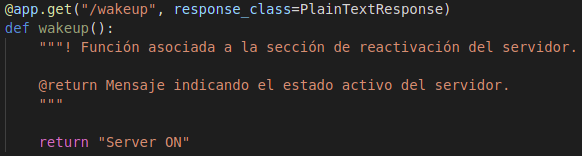
\includegraphics[width=0.7\textwidth]{imagenes/07_Implementacion/ejem_def_sec_servidor.png}
\caption{Ejemplo de definición de sección del servidor del Controlador}
\label{fig:ejem_def_sec_servidor}
\end{figure}

\subsection{Despliegue del servidor} \label{subsec:despl_servidor_heroku}

Como se ha indicado en la exposición de las herramientas del Controlador (Apartado \ref{subsec:herramientas_controlador}). Para el despliegue se hace uso principalmente de tres herramientas.

La primera herramienta a utilizar es Uvicorn. Uvicorn es un servidor ASGI basado en uvloop y httptools. Una hemos creado nuestro servidor con FastAPI, empleamos el mismo objeto con el que definíamos las secciones del servidor para ejecutar el servidor. Ayudándonos de la librería de Python de Uvicorn, utilizamos la función \textit{run} para ejecutar nuestro servidor FastAPI, pasándole como argumentos el objeto que define a la aplicación de FastAPI, el puerto en el que el servidor escuchará y la dirección de host. El puerto y la dirección host se pueden obtener tanto del archivo de configuración del servidor como de las variables de configuración de nuestra app en Heroku. Con esta información podremos ejecutar la aplicación de FastAPI mediante el módulo Uvicorn.

Pero hasta este punto únicamente tendríamos un servidor ejecutándose de forma local, situación que no es la conveniente para nuestro sistema, dado que uno de sus objetivos es que pueda ser empleado por cualquier persona y en cualquier momento. Es por ello que en este punto entra en acción el uso de una plataforma como es Heroku, herramienta analizada en el Apartado \ref{subsec:recur_software}. Y de la mano de Heroku viene la utilización de la herramienta Docker.

Heroku es una plataforma de tipo \gls{PaaS} que permite a los desarrolladores implementar, ejecutar y trabajar con aplicaciones que se estén ejecutando en su totalidad en la nube. De esta manera, al ejecutar nuestro servidor en esta plataforma, dispondremos de un punto de acceso público a nuestro sitio web y a todas las funcionalidades que proporciona.

Una vez sabemos de qué se trata la plataforma Heroku, debemos concretar como se traspasa nuestro trabajo realizado de forma local en nuestra máquina a un espacio de trabajo en la nube.

El despliegue a la plataforma de Heroku se realiza mediante la creación de un contenedor del servidor y su posterior subida a una de las apps que tengamos en nuestra cuenta de Heroku. Para obtener información más detallada sobre el proceso de despliegue en la plataforma Heroku puedes consultar el Apartado \ref{sec:proce_despli_server_Heroku}.


\subsection{Gestión del sitio web} \label{subsec:gest_sitio_web}

Una de las ventajas de usar FastAPI para la implementación del servidor es la posibilidad de utilizar cualquier motor para las plantillas HTML. Para el caso de nuestro servidor he optado por Jinja2, que es el motor que se recomienda en la documentación de FastAPI y el cual es frecuentemente empleado en otros \glspl{framework}. El único requisito para el uso de este gestor de plantillas es la instalación de la librería de Python \textit{jinja2}.

Para un fácil empleo de este gestor aparecen ejemplos de uso del mismo en la documentación de FastAPI \footnote{\url{https://fastapi.tiangolo.com/advanced/templates}}.

Para hacer uso del gestor en nuestro servidor es necesario seguir los siguientes pasos:

\begin{itemize}
\item Importar Jinja2Template de la librería fastapi.templating\ .
\item Montaje de los archivos de la carpeta static, carpeta cuyo contenido es todo aquel distinto de las plantillas HTML.
\item Creación del objeto templates con el cual se podrán manejar las plantillas
\item Declaración de un parámetro de tipo Request en cada una de las funciones asociadas a una ruta que devuelve una plantilla HTML. Además, cada una de estas funciones debe devolver una plantilla.
\item Generación de una plantilla renderizada mediante el objeto templates obtenido en el tercer paso.
\end{itemize}

Para conocer como se realiza el proceso de generación de las plantillas renderizadas puedes consultar el Apartado \ref{sec:proce_gen_plantillas}.

Con lo comentado hasta este momento podríamos tener un servidor web totalmente funcional en cuanto a lo estético, pero para poder realizar algunas de las funcionalidades del sitio web es necesario hacer uso de las posibilidades que nos da el gestor Jinja2 con el paso de valores a través del diccionario que se comenta en el Apartado \ref{sec:proce_gen_plantillas}. A través de este diccionario se pasará la información que requieran las plantillas y el cual no se pueda saber de forma estática, sino dinámica. Algunos ejemplos de este tipo de información pueden ser el estado del modo oscuro, es decir, si está activado o no; o la URL del servidor GPU, la cual puede cambiar durante la ejecución del Controlador si se inicia varias veces el servidor del Modelo durante la ejecución del servidor del Controlador.

Aunque para acceder a esta información desde los scripts de Javascript se deberá hacer de una manera menos directa a como puede parecer. Para conocer en más profundidad el proceso seguido para solucionar la dificultad de acceso a esta información desde los scripts, puedes consultar el Apartado \ref{sec:paso_info_scripts}.

\subsection{Secciones adicionales del servidor}

En este apartado se abordan las secciones del servidor del Controlador que no están orientadas al sitio web, sino que han surgido como solución a algún problema que haya surgido durante el desarrollo del servidor. En concreto, estamos hablando de dos secciones. Por un lado, una sección para la reactivación del servidor cada cierto tiempo; y, por otro lado, una sección para la actualización de la URL pública del servidor del Modelo.

\subsubsection*{Sección para la reactivación del servidor}

Por supuesto, la versión gratuita de Heroku tiene sus inconvenientes, principalmente enfocados en la actividad del servidor. El primer inconveniente se trata de una limitación en el uso de los recursos que nos proporciona la plataforma. Como se indicó en el apartado de gestión del proyecto, la plataforma Heroku dispone de unas unidades llamadas dynos, que son las encargadas de ejecutar nuestras apps. Con la versión gratuita, que es la que estamos utilizando, disponemos de una cuota de 550 horas gratuitas de utilización de los dynos. Esta cuota se renueva mensualmente. Esta información se puede comprobar en la sección de la documentación de Heroku sobre el empleo de los dynos gratuitos \footnote{\url{https://devcenter.heroku.com/articles/free-dyno-hours#usage}}. Además, esas 550 horas son horas de utilización con un único dyno, en el caso de usar dos dynos para nuestra app, dispondríamos de 275 horas gratuitas en total, es decir, la mitad. Si comparamos esta cantidad de horas, 550 horas, con la cantidad de horas de las que dispone como máximo un mes, las cuales son 744 horas, vemos como el número de horas que nos proporciona la versión gratuita se queda corta para poder proporcionar un servicio continuo del servidor. En el caso de que nuestra app supere la cuota de uso de nuestra cuenta, todos los dynos que estén ejecutando nuestras apps entrarán de forma forzosa en estado inactivo, dejando sin servicio a todas nuestras hasta que se vuelve a renovar la cuota de uso.

Para poder superar esta diferencia de horas sin tener llegar al apagado forzoso de los dynos, debemos hallar una solución para aumentar nuestra cuota de uso hasta llegar a una cuota que nos permita dar un servicio continuo. La plataforma Heroku nos da la posibilidad de aumentar esta cantidad de horas simplemente introduciendo los datos de la tarjeta de crédito en nuestra cuenta, sin tener que realizar ningún pago. La plataforma nos dará 1000 horas por el simple hecho de introducir estos datos. De esta manera superamos las 744 horas que puede tener como máximo un mes del año.

Un \gls{tip} que es interesante para llevar el control del consumo de nuestra cuota de utilización de los dynos es hacer uso de Heroku CLI mediante el comando \textit{heroku ps -a name&gt;}, con el cual obtendremos el porcentaje de la cuota que ya ha sido usado y el número de horas restante de la cuota. Aunque alternativamente se puede controlar este consumo de la cuota desde el apartado de pagos de nuestra cuenta, por si el administrador del sistema le es más agradable tener una interfaz gráfica para realizar este control.

Pero si analizamos el primer inconveniente, vemos como no tiene influencia en la implementación del servidor, y así es, aunque este no es el único inconveniente derivado del uso de la cuenta gratuita. El otro inconveniente de este tipo de cuentas es que los dynos que están ejecutando nuestro sitio web entran en estado inactivo al trascurrir cierto tiempo sin actividad en el servidor, de esta forma la plataforma no está gastando recursos de forma innecesaria. Esta desconexión de los dynos al no detectar actividad en la app se explican en la sección de la documentación de Heroku sobre la inactividad de los dynos \footnote{\url{https://devcenter.heroku.com/articles/free-dyno-hours#dyno-sleeping}}. Este paso a estado inactivo es un problema, ya que cuando se vuelve a tener actividad en el servidor se deberá volver a iniciar el servidor, lo que conllevará una espera que no será agradable para el usuario. A diferencia del primer inconveniente, Heroku no nos proporciona una solución a este segundo inconveniente, por lo que habrá que buscar una solución provisional para este inconveniente. Para más detalles sobre la solución a esta problemática, ver el Apartado \ref{sec:inactividad_Heroku}.

Después de aplicar estas dos soluciones tendremos un servidor disponible en cualquier momento.

\subsubsection*{Sección para la actualización de la URL pública del servidor del Modelo}

La gestión de la actualización de la URL pública del servidor es de igual forma importante para asegurar un servicio continuo del sitio web. Ya que puede darse el caso de que el servidor del Modelo se reinicie por cualquier motivo y cambie la URL pública del servidor. Esto sucede porque la URL pública del servidor se genera nuevamente cada vez que se inicia el servidor y cada vez que se genera es distinta. Esto sucede por la forma en que se ha implementado, lo cual se explicará en la sección de implementación del Modelo (Apartado \ref{sec:implementacion_modelo}).

Para gestionar este cambio dinámico de la URL, se ha creado una sección en el servidor del Controlador, donde se actualiza la variable que contiene la URL pública del servidor del Modelo. Esta sección se llama \textit{setURL}. Esta sección recibirá peticiones POST del servidor del Modelo, cuando se necesite actualizar la URL. Se necesitará actualizar la URL en los siguientes casos:

\begin{itemize}
\item Inicio del servidor del Modelo
\item Reinicio del servidor del Modelo
\item Inicio o reinicio del servidor del Controlador cuando el servidor del Modelo ya está activo.
\end{itemize}

Con el último caso descrito se deberá ejecutar una sección del servidor del Modelo para realizar la actualización. Este proceso se describirá en la sección de implementación del Modelo (Apartado \ref{sec:implementacion_modelo}).

La lógica de la sección generada es simple. Únicamente se recibe una petición POST que contiene la URL pública del servidor del Modelo, se extrae esa URL de la petición y finalmente se asigna el valor de la URL a la variable que contendrá el valor de la misma para poder ser usado por el resto de secciones del servidor.


\subsection{Procesado de las imágenes}

El procesado de las imágenes se realiza de forma distinta dependiendo del dispositivo que se esté utilizando. Aunque todo el procesado de las imágenes realizado por el Controlador se ha implementado en scripts de Javascript.

Si se usa un móvil, esta sección únicamente se compone de una parte, dado que el mismo botón de captura de la imagen lanza el envío de la imagen. Al pulsar sobre el botón de captura se lanzará la aplicación del sistema, la cual se encarga de capturar una imagen y preguntar al usuario si quiere utilizar esa imagen para la deducción de la edad. Una vez hemos aceptado cuál será nuestra imagen, el usuario será preguntado por el sistema por el permiso para el envío de la imagen. Si el usuario acepta el envío, se procederá a realizar el mismo. El envío consistirá en la lectura de la imagen en formato base64, seguido del envío de la imagen dentro de una petición POST a la ruta de deducción de edad del servidor del Modelo. Como respuesta a esta petición obtendremos el rango de edad que se ha deducido. Dependiendo de este rango de edad se abrirá una interfaz u otra, pero también habrá que tener en cuenta el canal que ha elegido el usuario. El canal elegido, la URL del servidor del Modelo, y la dirección a cada una de las interfaces disponibles se pasará al script a través del paso de valores con el módulo Jinja2, tal y como se indica en el Apartado \ref{subsec:gest_sitio_web}.

En el caso de usar otro dispositivo distinto del móvil, esta sección estará compuesta de dos partes. En la primera parte se realiza el mismo proceso que se realiza en la aplicación del sistema en el caso del móvil, aunque en este caso en vez de ver la imagen en la aplicación de captura de imágenes del sistema, se verá un elemento que mostrará el vídeo captado por la cámara del dispositivo y otro elemento que será un \gls{canvas} que almacenará la imagen que se captura del vídeo mencionado, ya que un vídeo no deja de ser una visualización continua de muchas imágenes. Una vez hemos capturado la imagen y la tenemos en el \gls{canvas}, tendremos un botón para iniciar el envío de la imagen. Este botón lanza la misma ventana que en el otro caso para pedir el permiso de envío de la imagen. El envío de la imagen se efectúa de forma similar a como se hace en el otro caso, cambiando únicamente la forma en que se obtiene la imagen, ya que en vez de leer la imagen de un archivo, se debe extraer la imagen almacenada en el \gls{canvas} y pasarla a formato base64. La información externa que se necesita para realizar el envío se obtiene de igual forma con el paso de valores con el módulo Jinja2.

\subsection{Gestión de la conversación}

La manera de gestionar la conversación por parte del Controlador está muy condicionada por el uso de las interfaces que proporciona Dialogflow. Dado que, como se ha mencionado en la implementación de la Vista, todo lo que sucede dentro de la interfaz no se puede controlar, ni siquiera los mensajes. Por ello se debe hacer uso de una funcionalidad que tiene Dialogflow, que es el Webhook. En esta sección de Dialogflow se deberá introducir una URL que servirá como punto de conexión entre Dialogflow y el servidor que funcione como webhook del chatbot. La URL que se colocará será aquella que nos lleve a la sección de webhook del servidor del Controlador. Habrá una sección de webhook por cada rango de edad, ya que habrá que gestionar por separado las interfaces de adulto y de niño. En cada uno de los Intents del chatbot de Dialogflow se activará la llamada al webhook, de esta forma cuando se active uno de los Intent se realizará el envío de una petición POST al webhook. Esta petición contendrá información de la conversación, como puede ser el Intent que se ha activado, el texto de entrada que ha activado al Intent o el contexto del chatbot.

Para conocer en detalle como se realiza la gestión de las peticiones recibida desde Dialogflow puedes consultar el Apartado \ref{sec:proce_gestion_conver}.

\subsection{Guardado de la conversación en el log} \label{subsec:guardado_conver}

Para facilitar la implementación del log de nuestro sistema, se ha hecho uso de las múltiples funcionalidades que proporciona Heroku a través de sus \gls{Add-ons}. En concreto, existe el \gls{Add-ons} llamado Heroku Postgres, el cual crea una base de datos Postgres que es accesible desde la app de Heroku, y que hará la función de log del sistema. Este \gls{Add-ons} se puede añadir de forma gratuita a nuestra app. Al instalar este \gls{Add-ons} se añade de manera automática la URL del log a las variables de configuración de nuestra app. Este último punto es importante, ya que será necesaria esta URL para realizar las conexiones con el log desde nuestro código del servidor del Controlador.

Para conocer como se realiza la conexión entre el servidor y el log a nivel de código puedes consultar el Apartado \ref{sec:conexion_server_log}.

Como se indicó en el diseño del Controlador, la duración de la conversación era un atributo calculado. Para obtener su valor se ha creado un disparador que se activa cada vez que se realiza una inserción en la tabla de las conversaciones. Este disparador activa una función que recibe la fecha de inicio y la fecha de fin de la conversación y calcula el tramo de tiempo que ha durado la conversación.

\section{Implementación del Modelo} \label{sec:implementacion_modelo}

\subsection{Herramientas para el desarrollo}

Las herramientas usadas en el Modelo, al igual que pasa en el Controlador, son muy diversas. Aunque hay ciertas herramientas que coinciden en ambas partes del sistema.

Toda la implementación del Modelo se realizará con el lenguaje de programación Python. La versión de Python utilizada será la versión 3.9.10.

Las herramientas comunes se encuentran en la sección de implementación y despliegue del servidor del Modelo. En cuanto a la implementación de la estructura del servidor, se hace empleo del \gls{framework} FastAPI. Para el despliegue, a diferencia de lo que pasa con el Controlador, se deja de utilizar la herramienta Docker. Aunque se podría usar la herramienta Docker en caso de que fuese útil para una mejora de la calidad del sistema. La herramienta que si se emplea para el despliegue del servidor es la herramienta Uvicorn. Otra herramienta que no se emplea para el despliegue es la plataforma Heroku. No se hace uso de esta plataforma por la simple razón de que no dispone de apps con servicio de GPU. Por ello, para realizar el despliegue del servidor del Modelo se ha empleado la herramienta Ngrok, para realizar el despliegue de forma local en el servidor GPU del Instituto DaSCI y poder generar un punto de acceso público al servidor del Modelo.

Una parte fundamental del Modelo es la generación de respuestas, ya que es básica para la elaboración del chatbot. Como se ha comentado en el diseño del Modelo, esta generación de respuestas se va a basar en modelo pre entrenados del chatbot BlenderBot. Es en este punto cuando interviene el uso de la plataforma Huggingface \footnote{\url{https://huggingface.co/}}. Esta plataforma sirve como una base de modelos que son subidos por la comunidad. El modelo pre entrenado utilizado para toda la generación de respuestas es el modelo \href{https://huggingface.co/facebook/blenderbot-400M-distill}{blenderbot-400M-distill} de la empresa Facebook.

Si nos fijamos en el lenguaje empleado por el modelo de generación de respuestas, vemos que trabaja con texto en inglés, por lo tanto, será necesario traducir el texto de español a inglés y viceversa. Para nuestro sistema hemos empleado la API de DeepL, la cual nos permite tener un traductor varias veces mejor que el resto de traductores disponibles actualmente.

Otra sección del Modelo que ha hecho uso de la plataforma Huggingface, es la deducción de la edad a través de imágenes. Para reducir el tiempo de desarrollo del sistema sin dejar tener un sistema fiable, he optado por usar un modelo pre entrenado de clasificación de imágenes, el cual es capaz de clasificar una imagen de una persona en un rango de edad concreto. El modelo utilizado es \href{https://huggingface.co/nateraw/vit-age-classifier}{vit-age-classifier} del desarrollador nateraw.

\subsection{Implementación del servidor}

Dado que en la sección de herramientas se ha indicado que la implementación de la estructura del servidor se realizaría con el \gls{framework} FastAPI, la implementación llevada a cabo para el servidor del Modelo no diferirá mucho de la implementación del servidor del Controlador, la cual se puede ver en el Apartado \ref{subsec:implementacion_controlador}. Una de las diferencias será el número y la funcionalidad de las secciones del servidor, y la otra diferencia estará relacionada con el intercambio de información entre los servidores. Esta última diferencia viene originada por la propia estructura de nuestro sistema, ya que debemos implementar dos servidores con dominio distinto que se comunican entre ellos. Este intercambio de información tiene especial importancia en las comunicaciones entre la interfaz y el servidor del Modelo. Dado que la interfaz del sistema se encuentra en el dominio del servidor del Controlador y el servidor del Modelo se encuentra en un dominio distinto, deberemos añadir ciertas cabeceras en las conexiones entre ambas partes del sistema.

Para obtener una información detallada de las cabeceras añadidas a las conexiones con el servidor del Modelo, puedes consultar el Apartado \ref{sec:cabecera_conexion_Modelo}.

\subsection{Despliegue del servidor}

Para el despliegue del servidor se hace uso de dos herramientas, una de ellas ya empleada para el despliegue del servidor del Controlador.

La herramienta que ya ha sido utilizada es Uvicorn. Esta herramienta, como ya se explicó en el despliegue del Controlador, es un servidor ASGI el cual nos permite poner en funcionamiento la estructura de nuestro servidor, la cual se ha creado con FastAPI. Para poner en funcionamiento el servidor será necesario definir el puerto y la dirección host que empleará el módulo Uvicorn.

Llegados a este punto tenemos un servidor ejecutando de forma local, por lo tanto, no hay forma de acceder al servidor desde el exterior del sistema. A diferencia de lo aplicado con el servidor del Controlador, no se hará uso de la plataforma Heroku, dado que necesitamos tener disponibles GPU's para la utilización de los modelos basados en Transformers. Por ello debemos mantener el servidor ejecutando de forma local, pero no en nuestra máquina, sino en el \href{https://dasci.es/es/sobre-dasci/recursos/recursos-tecnologicos/}{servidor GPU del Instituto DaSCI}. Pero nos apoyaremos en la herramienta Ngrok para posibilitar un acceso público al servidor del Modelo. Ngrok es un servicio que permite el acceso a un servidor a través de internet, creando el servidor local en un subdominio.

Dado que para la implementación se hace empleo del lenguaje Python, no se usará la herramienta Ngrok en sí, sino una librería de Python llamada pyngrok \footnote{\url{https://github.com/alexdlaird/pyngrok}}.

Una vez que sabemos con qué vamos a posibilitar el acceso al servidor, falta detallar la manera en que se hará. El proceso seguido para desplegar el servidor mediante la herramienta Ngrok se explica detalladamente en el Apartado \ref{sec:proce_despli_server_Modelo}.

\subsection{Generación de los conjuntos de datos} \label{subsec:gen_conj_datos}

Por supuesto que los modelos que generan las respuestas del chatbot son una parte principal del sistema, pero no podemos disfrutar de ellos, si no disponemos de buenos conjuntos de datos con los que entrenar a los modelos.

Un conjunto de datos para entrenar un modelo conversacional consiste simplemente en una tabla con dos columnas, por un lado, las preguntas o entradas; y, por otro lado, las respuestas o salidas.

En un principio no disponíamos de información suficiente para crear un chatbot. Por esta razón optamos por extraer la información de la página Quora \footnote{\url{https://www.quora.com/}}. Esta fase es la más costosa tanto en tiempo como en dinero a la hora de crear un chatbot. La página Quora es una red social de preguntas y respuestas, donde existen conversaciones sobre distintos temas. Actualmente, existen ciertos módulos para la extracción de información especializados en esta página, pero en mi caso he optado por generar mi propio programa de extracción de información para obtener los conjuntos de datos con el formato deseado. Este programa extraerá la información de la página y generará una tabla con todos los datos extraídos. Para obtener más detalles de esta extracción de información se puede ver el Apartado \ref{sec:extraccion_info}.

Disponiendo de este programa ya podremos extraer un conjunto de datos inicial con información sobre los temas que nos interesen.

El conjunto de datos que obtendremos no tendrá el formato adecuado para ser usado por los modelos, por ello será necesario realizar un pre procesado al conjunto de datos. Además, como disponemos de dos modelos, uno para adultos y otro para niños, y únicamente tenemos un conjunto de datos. A la vez que ejecutamos el pre procesado deberemos tratar los textos del conjunto de datos de tal forma que se adapten al rango de edad al que van destinados. Por lo tanto, tras el pre procesado del conjunto de datos inicial obtendremos como resultados dos conjuntos de datos, uno para adultos y otro para niños. Ambos con el formato adecuado para ser utilizados por los modelos.

Para conocer cuál es el proceso seguido para realizar el pre procesado puedes consultar el Apartado \ref{sec:preprocesado_conj_datos}.

\subsection{Entrenamiento de modelos}

El siguiente paso lógico, tras haber generado los conjuntos de datos, es el entrenamiento de los modelos pre entrenados mediante los conjuntos de datos obtenidos. Como ya se ha indicado en anteriores apartados, el entrenamiento de nuestros modelos consistirá en un ajuste de los mismos, es decir, en un entrenamiento de unas pocas épocas. Para realizar el ajuste se elaborará un programa que realizará este proceso. Durante la ejecución del programa se irá mostrando por pantalla información detallada sobre el estado del proceso. Esta información va desde la época en que nos encontramos hasta las métricas obtenidas en ese punto del entrenamiento.

Por supuesto, lo primero que debemos hacer si queremos entrenar unos modelos es efectuar la carga de los mismos. Un modelo se compone de tres partes principales, su configuración, su tokenizer, que es el módulo encargado de pasar de texto a lista de tokens y viceversa; y el propio modelo.

Y en segundo lugar, debemos cargar otras de las partes fundamentales para el entrenamiento, los conjuntos de datos. Se deben cargar los conjuntos de datos de entrenamiento y validación del rango de edad que se quiera aplicar al modelo cargado previamente. Estos conjuntos de datos pueden ser cargados en su totalidad o parcialmente. Pero tras la carga no termina el trabajo con los conjuntos de datos, dado que los modelos trabajan con tokens no con cadenas de caracteres. Entonces debemos aplicar un pre procesado a los conjuntos de datos cargados, para tener conjuntos de datos cuyo contenido sean tokens.

Una vez tenemos todos los elementos para proceder al entrenamiento, debemos crear el objeto que realiza el entrenamiento, el cual hará uso de todos los elementos anteriormente descritos. Este entrenador será el encargado de ir entrenando el modelo cargado basándose en las métricas que vaya obteniendo. El cálculo de las métricas se efectuará en cada época, al igual que el guardado de modelos. Finalmente, se guardará el mejor modelo encontrado durante el proceso de ajuste, al igual que las métricas obtenidas con ese modelo.

Este programa podrá también evaluar el modelo cargado, guardando las métricas obtenidas.

Todas las métricas obtenidas durante todo el programa se guardarán en un archivo para su posible análisis futuro.

La métrica utilizada para guiar todo el proceso de entrenamiento ha sido la métrica BLEU. BLEU (Bilingual Evaluation Understudy) es un algoritmo para evaluar la calidad de un texto traducido por una máquina de una lengua natural a otra. Se considera que la calidad es la correspondencia entre el resultado de una máquina y el de un humano. Cuanto más se acerque una traducción automática a una traducción humana profesional, mejor será. El BLEU fue una de las primeras métricas en afirmar una alta correlación con los juicios humanos sobre la calidad, y sigue siendo una de las métricas automatizadas más populares y económicas.

Las puntuaciones se calculan para segmentos individuales traducidos, comparándolos con un conjunto de traducciones de referencia de buena calidad. A continuación, esas puntuaciones se promedian en todo el corpus para obtener una estimación de la calidad global de la traducción. No se tienen en cuenta ni la inteligibilidad ni la corrección gramatical.

\subsection{Generación de respuestas}

La generación de las respuestas se realiza en dos secciones distintas del servidor del Modelo, una por cada rango de edad que tiene disponible el chatbot. Estas secciones serán las encargadas de recibir las peticiones del Controlador, generar la respuesta y devolver esa respuesta como respuesta a la petición del Controlador. Por supuesto, antes de iniciar el servidor deberemos cargar los modelos de los distintos rangos de edad. Esta carga se hará mediante la función \textit{from\_pretrained}, para asegurarnos de que únicamente un proceso pueda cargar el modelo y el vocabulario al mismo tiempo. Para esta sección se hará uso de dos herramientas adicionales. La primera herramienta son los pipelines, en nuestro caso los pipelines conversacionales. Estos pipelines facilitan la generación de respuestas al poder crear instancias de las conversaciones, las cuales guardan un registro de las entradas y sus correspondientes respuestas más recientes. La segunda herramienta, y puede que la más importante de este módulo, es el módulo \href{https://deepspeed.readthedocs.io/en/latest/}{deepspeed}. Este módulo es un optimizador de los modelos basados en Transformers. Este módulo permite que la generación de respuestas se haga de forma casi instantánea, permitiendo una respuesta del chatbot en un tiempo muy breve. Para realizar esta optimización se pasan todos los modelos utilizados en los pipelines por este módulo, mediante la función \textit{init\_inference}. Una funcionalidad que no se ha usado de este módulo, pero la cual se podría llegar a usar, es el uso conjunto de varias GPU's para la generación de respuestas. Para nuestro proyecto únicamente se hace uso de una GPU.

La petición del Controlador no contiene únicamente el texto de entrada, sino también el identificador de la conversación y un indicador para saber si se trata de la última respuesta de la conversación.

La generación de respuestas consistirá en los siguientes pasos:

\begin{itemize}
\item Traducir al inglés el texto recibido en la petición del Controlador
\item Obtener la conversación actual mediante su identificador
\item Añadir el texto traducido como entrada a la conversación obtenida
\item Generación de la respuesta mediante el pipeline
\item Actualización de la conversación añadiendo la respuesta generada
\item Traducir al español la respuesta
\item Elaborar la respuesta a la petición del Controlador
\end{itemize}

Por último, cabe destacar que la generación llevada a cabo por el pipeline se basa en una serie de parámetros, lo cuales serán definidos en la configuración del proceso de ajuste. Principalmente, la generación se basa en dos parámetros, \textit{temperature} y \textit{top\_p}. Ambos parámetros modifican la flexibilidad del chatbot a la hora de generar texto.

Un punto a destacar, que no se puede pasar por alto es la gestión del historial de las conversaciones, ya que para que la generación de respuestas tenga sentido se debe tener un historial de la conversación. Este historial se va generando a través de los resultados que van devolviendo los pipelines durante la generación de las respuestas. Pero para poder identificar cada conversación con un usuario se debe mantener un control de las mismas, puesto que las peticiones al servidor del Modelo no van en un principio enlazadas con ninguna conversación. Este control se realiza mediante un diccionario, cuya clave es el identificador de la conversación. Este diccionario se irá actualizando conforme vayan progresando las conversaciones activas en el sistema. El identificador de la conversación se irá trasmitiendo junto a las peticiones que efectúe el Controlador, y finalmente en la última respuesta se eliminará la entrada asociada a la conversación indicada en la petición.

\subsection{Deducción de edades}

A lo largo de la implementación del Modelo se ha visto como se hace diferenciación según el rango de edad del usuario, pero todavía no hemos visto como llegamos a saber cuál es el rango de edad del usuario.

Antes de comenzar con la explicación sobre como se realiza la deducción, cabe destacar dos aspectos importantes en esta deducción. En primer lugar, el límite de edad entre el rango de edad de niño y de adulto se encuentra a los 12 años. Para nuestro sistema un niño tendrá como máximo 12 años inclusive. Una vez sabemos como se dividen los rangos de edad en nuestro sistema, es el momento de indicar el segundo aspecto. Este segundo aspecto son los distintos rangos de edad que el modelo pre entrenado utilizado, es capaz de clasificar. Los rangos de edad del modelo son los siguientes:

\begin{itemize}
\item 0 - 2 años
\item 3 - 9 años
\item 10 - 19 años
\item 20 - 29 años
\item 30 - 39 años
\item 40 - 49 años
\item 50 - 59 años
\item 60 - 69 años
\item Más de 70 años
\end{itemize}

Como se puede apreciar, el límite de edad entre los dos rangos de edad del sistema se encuentra incluido en el tercer rango de edad de clasificación del modelo. La solución a este problema se irá indicando conforme se explique la implementación de esta sección.

Una vez explicados estos dos aspectos comenzamos con la explicación de la implementación de la sección de deducción. Si el usuario dio permisos al sistema para usar imágenes, el Modelo recibirá peticiones desde el Controlador, las cuales contendrán imágenes del usuario. Estas imágenes no serán guardadas en ningún momento, para asegurar la privacidad de los usuarios; además, las peticiones con las cuales se envían las imágenes son totalmente seguras al ser del tipo HTTPS.

Como se ha indicado en el diseño del Modelo, para la deducción de la edad se hace uso de un modelo basado en Transformers, cuya funcionalidad es la clasificación de personas basándose en su edad.

En primer lugar, se deberá cambiar el formato de la imagen recibida en la petición para poder pasarla como entrada al modelo. Una vez tenemos la imagen en el formato adecuado, realizaremos la clasificación con el modelo. La salida del modelo será una lista de probabilidades. Esta lista tendrá tantos elementos como rangos de edad puede llegar a clasificar el modelo. Una vez tenemos esta lista, nos quedaremos con la mayor probabilidad. Para solucionar el problema de tener el límite en medio de un rango de edad se utilizará una heurística para decidir el rango de edad del usuario. Si la mayor probabilidad se encuentra en el primer o segundo rango, se indicará que es un niño. Si la mayor probabilidad se encuentra en el cuarto rango de edad o posteriores, se indicará que es un adulto. Y para el rango de edad restante, el tercer rango de edad, la decisión se basará en un cálculo. Se calculará la suma de las probabilidades desde el inicio de la lista hasta el tercer rango inclusive, y otra suma desde el tercer rango hasta el final de la lista inclusive. Si la primera suma es mayor o igual a la segunda se indicará que es un niño, en caso contrario se indicará que es un adulto. Con el uso de esta heurística deberíamos poder solucionar ese problema, pero no lo sabremos hasta que no hagamos pruebas con el sistema. Una vez se sabe el rango de edad a devolver, se realiza la devolución de la respuesta a la petición del Controlador.

